\documentclass[aspectratio=169]{beamer}
\usepackage{standalone}

\usepackage{stmaryrd}
\usepackage{listings}
\usepackage{fontawesome}
\usepackage{bm}

\usepackage[hyperref=auto,style=alphabetic,backend=bibtex]{biblatex}
\addbibresource{kwarcpubs.bib}
\addbibresource{extpubs.bib}
\addbibresource{extcrossrefs.bib}
\addbibresource{bib.bib}
\addbibresource{examples.bib}
\usepackage{appendixnumberbeamer}
\usepackage{tikz}
\usepackage{tikz-qtree}
\usetikzlibrary{arrows.meta}
\usetikzlibrary{shapes}
\usetikzlibrary{mmt}
\usetikzlibrary{docicon}

\usetheme{Pittsburgh}
% \setbeamertemplate{footline}[frame number]
\setbeamertemplate{footline}{\hfill\insertframenumber\,/\,\inserttotalframenumber\quad\strut}
\setbeamertemplate{navigation symbols}{}
\usecolortheme{beaver}
\setbeamertemplate{frametitle}[default][left]
% \setbeamersize{text margin left=3em}

\usepackage{utils/colors}
\usepackage[forbeamer]{utils/basic}
\usepackage{utils/operators}
\usepackage{utils/mylstmisc}
\usepackage{utils/lstmmt}

\lstset{basicstyle=\ttfamily}
\lstset{commentstyle=\itshape\color{commentfont}}
\def\examplecite#1{{\textit{\color{black!60!blue}\small Example from \cite{#1}}}}



% rdf nodes
\tikzset{urinode/.style={draw, ellipse, minimum width=1.3cm, minimum height=0.6cm}}
\tikzset{typenode/.style={draw}}
\tikzset{bnode/.style={draw, ellipse, minimum width=1.0cm, minimum height=0.6cm}}
\tikzset{literal/.style={draw, rounded corners=0.1cm}}

% rdf edges
\tikzset{normaledge/.style={-Latex}}
\tikzset{typeedge/.style={arrows={-Latex[open]}}}

% custom nodes
\tikzset{body/.style={fill=green!50}}
\tikzset{target/.style={fill=blue!30}}
\tikzset{annotation/.style={fill=red!50}}


\title{Annotating and Spotting in Mathematical Corpora\\(concepts and tools)}
\author{Jan Frederik Schaefer}
\institute{FAU Erlangen-N\"urnberg}
\date{\textbf{Prospects of Formal Mathematics -- Bridging between informal and formal}\\Hausdorff Research Institute for Mathematics\\Bonn\\July 10, 2024}

\begin{document}
\begin{frame}
    \frametitle{Natural Language Processing and Mathematical Language}
    \begin{itemize}
        \item Natural language processing has benefitted from a long tradition of annotation tasks and benchmarks
        \item STEM documents pose problems:
            formulae, tables, \textellipsis
            \com{not really unicode strings}
        \item Why care?\\
            $\leadsto$ Semantic services
    \end{itemize}
\end{frame}

\begin{frame}
    \frametitle{Accumulating semantic annotations with spotters}
    \centering
    \textbf{Spotter:} specialized tool for finding a particular type of annotation
    \vspace{2em}\par

    \begin{tikzpicture}[db/.style={cylinder, shape border rotate=90, draw, aspect=0.3,scale=4},spotter/.style={draw}]
        \node[db,thick] (db) at (0, 0) {};
        \node[spotter] (s1) at (-3, 1) {\begin{tabular}cParagraph\\classification\\spotter\end{tabular}};
        \node[spotter] (s2) at (3, 1.5) {\begin{tabular}cDeclaration\\spotter\end{tabular}};
        \node[spotter] (s3) at (3, -1.5) {\begin{tabular}cMath concept\\spotter\end{tabular}};
        \node[spotter] (s4) at (-3, -1.5) {\begin{tabular}cUnit\\spotter\end{tabular}};
        \draw[->] (s1) -- (db);
        \draw[->] (s2) -- (db);
        \draw[->] (s3) -- (db);
        \draw[->] (s4) -- (db);
        \node (doc) at (0, -4.5) {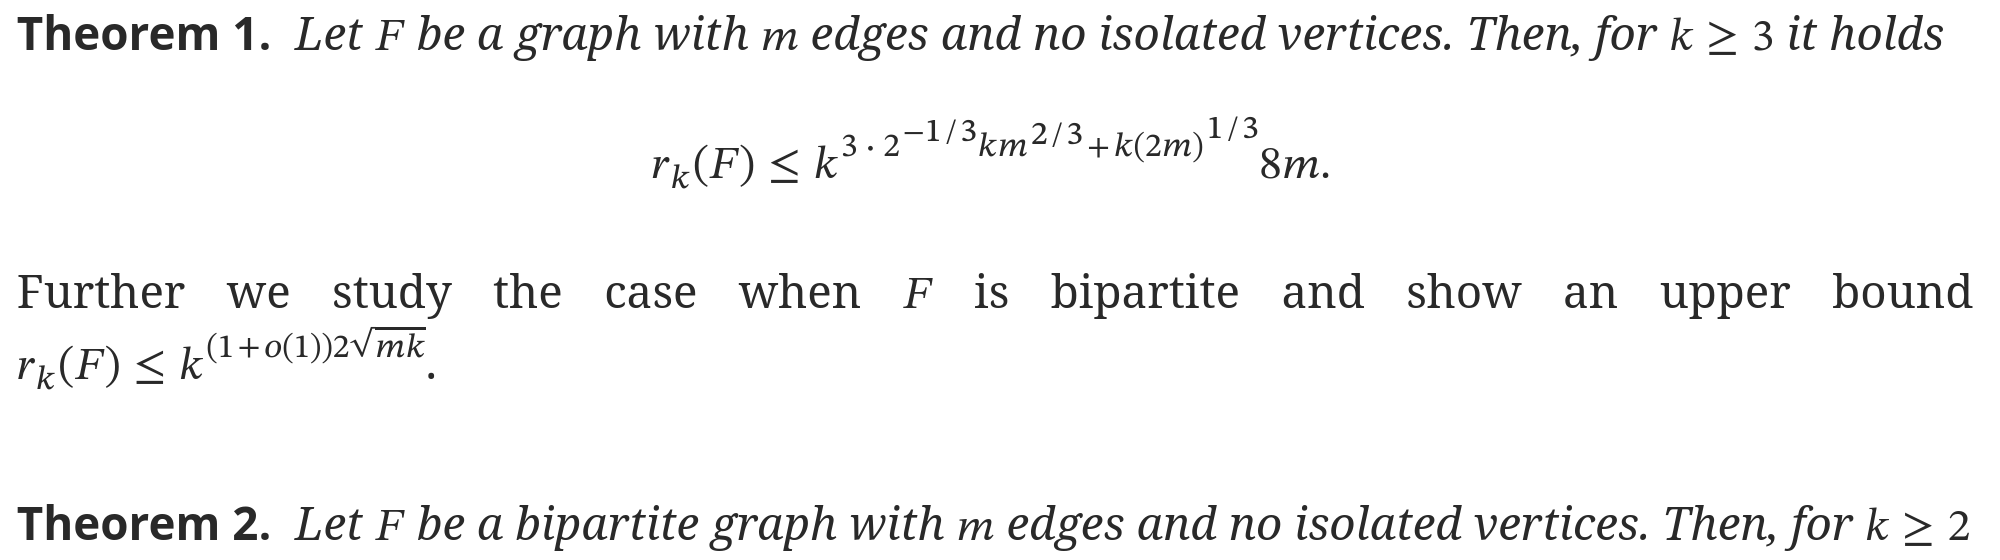
\includegraphics[scale=0.25]{theorems_1311_5471.png}};
        \node at (5, -4) {\examplecite{johst2013multicolor}};
        % \node[draw] (doc) at (0, -3) {\bf Fixed/frozen corpus};
        \draw[->,dashed] (db) -- (doc);
    \end{tikzpicture}

%     \begin{itemize}
%         \item \textbf{Spotter:} specialized tool for finding a particular type of annotation
%         \item Examples: Identifier declarations, quantity expressions,
%             paragraph type (theorem/definition/\textellipsis), \textellipsis
%         \item Simple spotters, hybrid spotters, meta spotters
%     \end{itemize}
    % pictures with annotations (simple spotter, hybrid spotter, meta spotter)
    % e.g. "concept references and quantities", "variable declarations", "conflict resolution var. occurrence vs unit"
\end{frame}


\begin{frame}
    \frametitle{What is the problem?}
    \begin{enumerate}
        \item Getting a corpus:\com{Working with PDF is difficult}
            \begin{itemize}
                \item arXMLiv/ar5iv dataset~\cite{SML:arXMLiv:2020}\com{convert \texttt{.tex} to \texttt{.html}}
                \item SIGMathLing~\cite{SIGMathLing:on}\com{NDA-cooperative to work around licensing issues}
            \end{itemize}
        \item Re-inventing the wheel:
            \begin{itemize}
                \item Need to obtain plaintext representation
                \item Need to store annotations
                \item Need to create manual annotations\com{for training/evaluation}
            \end{itemize}
        \item Cannot re-use existing annotations/combine results:
            \begin{itemize}
                \item No agreed-upon annotation format
                \item Original documents modified
            \end{itemize}
    \end{enumerate}
\end{frame}

\begin{frame}
    \frametitle{Annotation structure (following W3C Web Annotation Recommendation)}
    \centering
    % body, target, meta-data
    \begin{tikzpicture}[yscale=1.8]
        \node[urinode,annotation] (anno) at (0, 0) {ex:anno1};
        
        \node[typenode] (annot) at (-4.5, 1) {oa:Annotation};
        \draw[typeedge] (anno) --node[fill=white]{rdf:type} (annot);
        \node[urinode] (author) at (0, 1) {\textellipsis};
        \draw[normaledge] (anno) --node[fill=white,pos=0.4]{dcterms:creator} (author);
        \node[urinode] (created) at (4.5, 1) {\textellipsis};
        \draw[normaledge] (anno) --node[fill=white,pos=0.6]{dcterms:created} (created);

            \node (targ) at (-3, -1) {\textellipsis};
            \draw[normaledge] (anno) --node[fill=white]{oa:hasTarget} (targ);
            % \node[urinode] (targ) at (-3, -1) {ex:target1};
            % \draw[normaledge] (anno) --node[fill=white]{oa:hasTarget} (targ);
            % \node (targ1) at (-4,-1.5) {\textellipsis};
            % \node (targ2) at (-2,-1.5) {\textellipsis};
            % \draw[normaledge] (targ) -- (targ1);
            % \draw[normaledge] (targ) -- (targ2);

            % \node[urinode] (body) at (3,-1) {ex:body1};
            \node (body) at (3,-1) {\textellipsis};
            \draw[normaledge] (anno) --node[fill=white]{oa:hasBody} (body);
    \end{tikzpicture}
        \vspace{2em}\par
        \begin{columns}
            \begin{column}{0.5\textwidth}
                \centering
                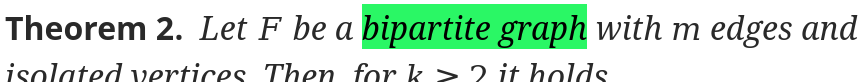
\includegraphics[width=\textwidth]{bipart_graph.png}
                \\\hfill\examplecite{johst2013multicolor}
            \end{column}
            \begin{column}{0.5\textwidth}
                \centering
                \texttt{wd:Q174733}\\
                (WikiData: bipartite graph)
            \end{column}
        \end{columns}
\end{frame}


\begin{frame}[fragile]
    \frametitle{Annotation Targets}
    \centering
    \footnotesize
    \begin{tikzpicture}[xscale=-1]
        \node[urinode,annotation] (anno) at (0, 0) {ex:anno0};
        \node[bnode,body] (body) at (-2, -1.3) {\textellipsis};
        \draw[normaledge] (anno) --node[fill=white]{oa:hasBody} (body);
        \node[urinode,target] (target) at (4, -1.5) {ex:target0};
        \node[urinode,target] (src) at (5, 0) {ex:document.html};
        \draw[normaledge] (anno) --node[fill=white]{oa:hasTarget} (target);
        \draw[normaledge] (target) --node[fill=white]{oa:hasSource} (src);

            \node[typenode,target] (pathseltype) at (7.2, -2.3) {sb:PathSelector};
            \node[bnode,target] (pathsel) at (5.2, -3.75) {};
            \node[literal,target] (pathselstart) at (2.5, -5.5) {``after-node(/html/.../math[3])''};
            \node[literal,target] (pathselend) at (7.5, -5.5) {``char(/html/.../p[2], 819)''};

            \draw[normaledge] (target) --node[fill=white]{oa:hasSelector} (pathsel);
            \draw[normaledge] (pathsel) --node[fill=white]{sb:startPath} (pathselend);
            \draw[normaledge] (pathsel) --node[fill=white]{sb:endPath} (pathselstart);
            \draw[typeedge] (pathsel) --node[fill=white]{rdf:type} (pathseltype);

            \node[typenode,target] (offseltype) at (0.5, -1.5) {sb:OffsetSelector};
            \node[bnode,target] (offsel) at (1, -3) {};
            \node[literal,target] (offselstart) at (2.3, -4.5) {1592};
            \node[literal,target] (offselend) at (0, -4.5) {1605};
            \draw[normaledge] (offsel) --node[fill=white]{oa:start} (offselstart);
            \draw[normaledge] (offsel) --node[fill=white]{oa:end} (offselend);
            \draw[normaledge] (target) --node[fill=white]{oa:hasSelector} (offsel);
            \draw[typeedge] (offsel) --node[fill=white]{rdf:type} (offseltype);
    \end{tikzpicture}
\end{frame}


\begin{frame}
    \frametitle{Questions}

    \begin{itemize}
        \item Is this the ``right'' approach?\com{scalability, \ldots}
        \item What kinds of annotation tasks are attractive and feasible?
    \end{itemize}
    \vspace{1em}
\end{frame}

\appendix   % stop page number count

\begin{frame}[allowframebreaks,t]
    \frametitle{References}
    \printbibliography
\end{frame}

\end{document}
